\documentclass[11pt,letterpaper]{exam}
\usepackage[utf8]{inputenc}
\usepackage{graphicx}
\usepackage{tabularx}
\usepackage[absolute]{textpos} % Para poner una imagen en posiciones arbitrarias
\usepackage{multirow}
\usepackage{float}
\usepackage{hyperref}
%\decimalpoint

\begin{document}
\begin{center}
{\Large Métodos Computacionales} 
\end{center}


\noindent
\section{Ejercicio 1: Fourier} 
\vspace{5mm}
\subsection{    Gráficas usando funciones signal and signalSuma.} 
\vspace{5mm}
\begin{center}
\includegraphics[width=10cm]{GarzonCamilo_signal_signalSuma.pdf} 

Figura 1. Grafica signal y signalSuma.

\includegraphics[width=10cm]{GarzonCamilo_TransformadasFourier_signal_signalSuma.pdf} 

Figura 2. Grafica transformada discreta de fourier de signal y signalSuma.
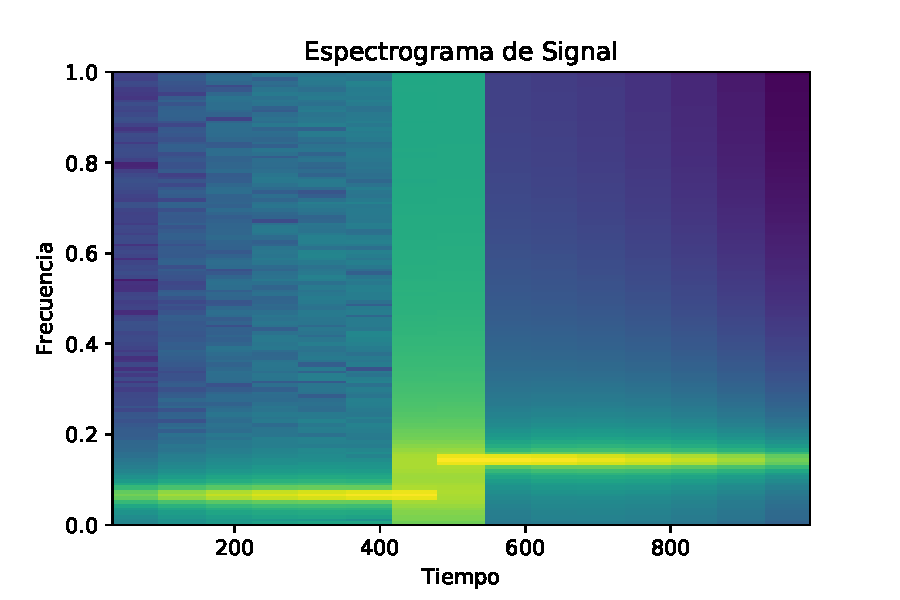
\includegraphics[width=10cm]{GarzonCamilo_espectograma_signal.pdf} 


Figura 3. Espectograma de la función signal .
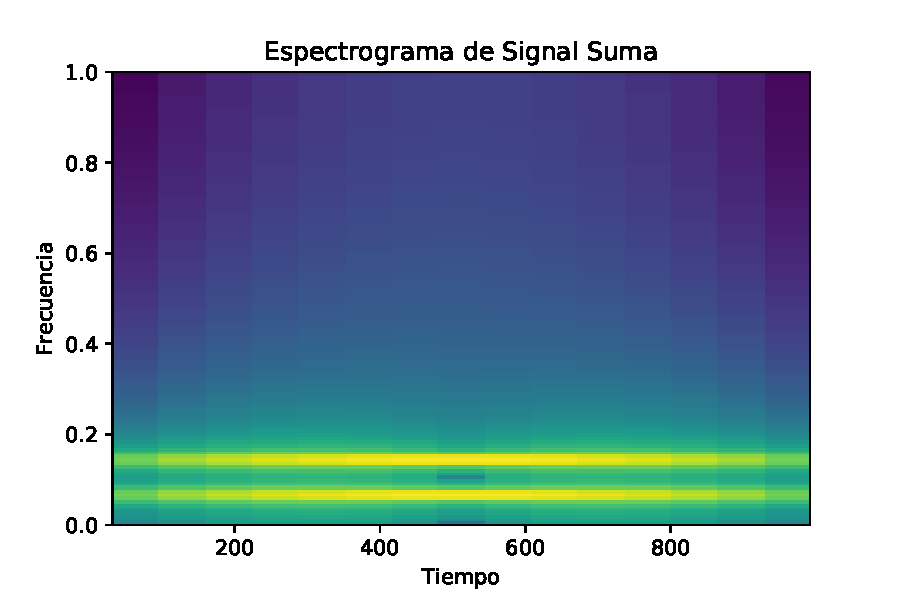
\includegraphics[width=10cm]{GarzonCamilo_espectograma_signalSuma.pdf} 


Figura 4. Espectograma de la función s signalSuma.
\end{center}
\vspace{5mm}
\subsection{    Gráficas usando la funcion de un temblor.} 
\vspace{5mm}
\begin{center}
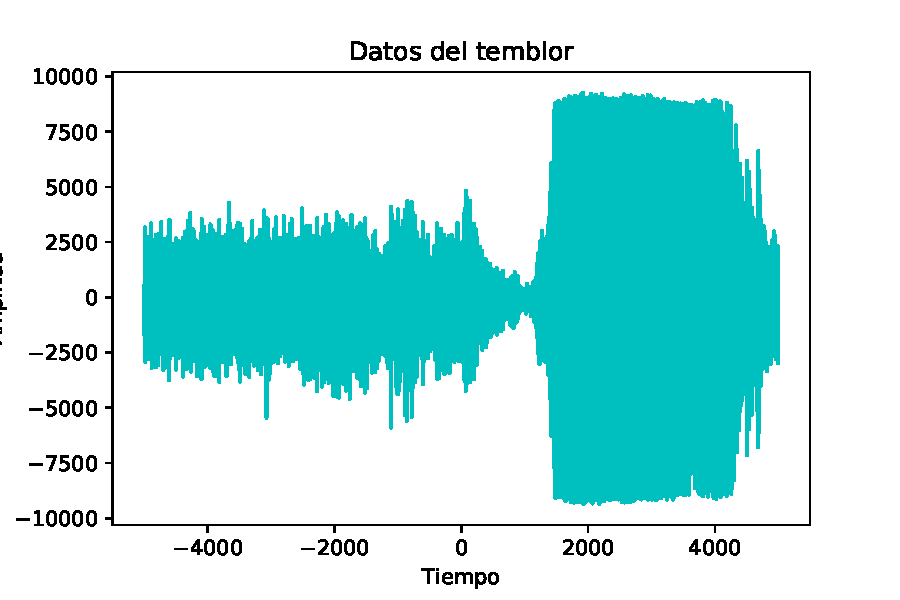
\includegraphics[width=10cm]{GarzonCamilo_temblor.pdf} 

Figura 5. Grafica temblor.

\includegraphics[width=10cm]{GarzonCamilo_TransformadasFourier_temblor.pdf} 

Figura 6. Grafica transformada discreta de fourier de la función del temblor.
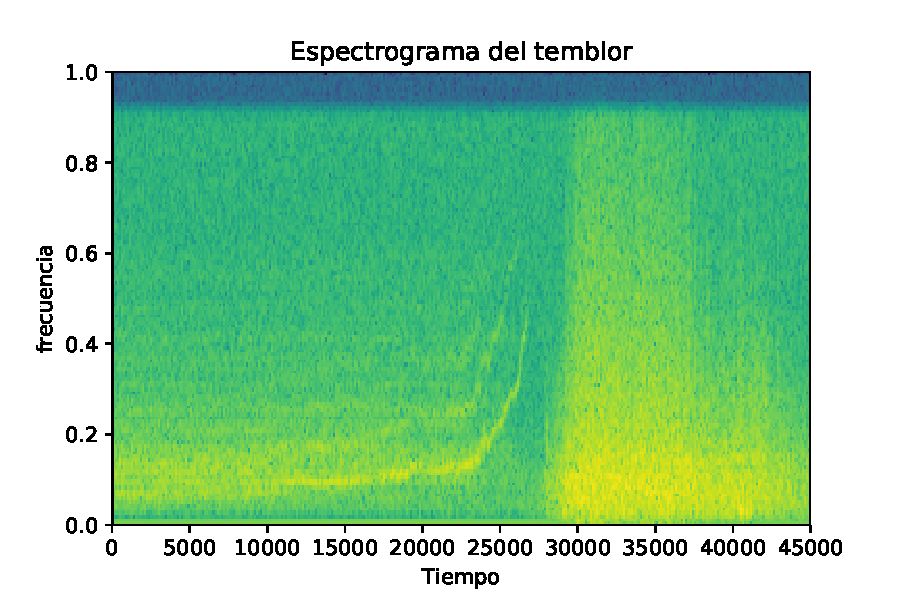
\includegraphics[width=10cm]{GarzonCamilo_espectograma_temblor.pdf} 

Figura 7. Espectograma de la función del temblor.
\end{center}

\end{document}

